Codeigniter adalah sebuah framework untuk web yang dibuat dalam format PHP. Format yang dibuat ini selanjutnya dapat digunakan untu membuat sistem aplikasi web yang kompleks. Codeigniter dapat mempercepat proses pembuatan web, karena semua class dan modul yang dibutuhkan sudah ada dan programmer hanya tinggal menggunakannya kembali pada aplikasi web yang akan dibuat \cite{prabowo2015website}.

\section{Tutorial Install CodeIgniter 3}
    \begin{enumerate}
        \item Pertama download Framework CodeIgniter di \textbf{\textit{https://www.codeigniter.com/}}
        
	    \item Setelah mengunduh file CodeIgniter 3, ekstrak file tersebut menggunakan WinRAR atau 7Zip kedalam folder htdocs jika kamu menggunakan XAMPP atau \textit{/var/www/html}. jika kamu menggunakan Apache2 Standalone, setelah itu ubahlan nama foldernya menjadi namaapplikasi.
	    
	    \item Sekarang silahkan Kamu coba akses URL \textbf{\textit{http://localhost/ namaaplikasi/}} melalui browser Kamu, akan langsung ditampilkan halaman awal Codeigniter yang berarti Instalasi telah berhasil.
		\begin{figure}[!htbp]
    		\centering
    		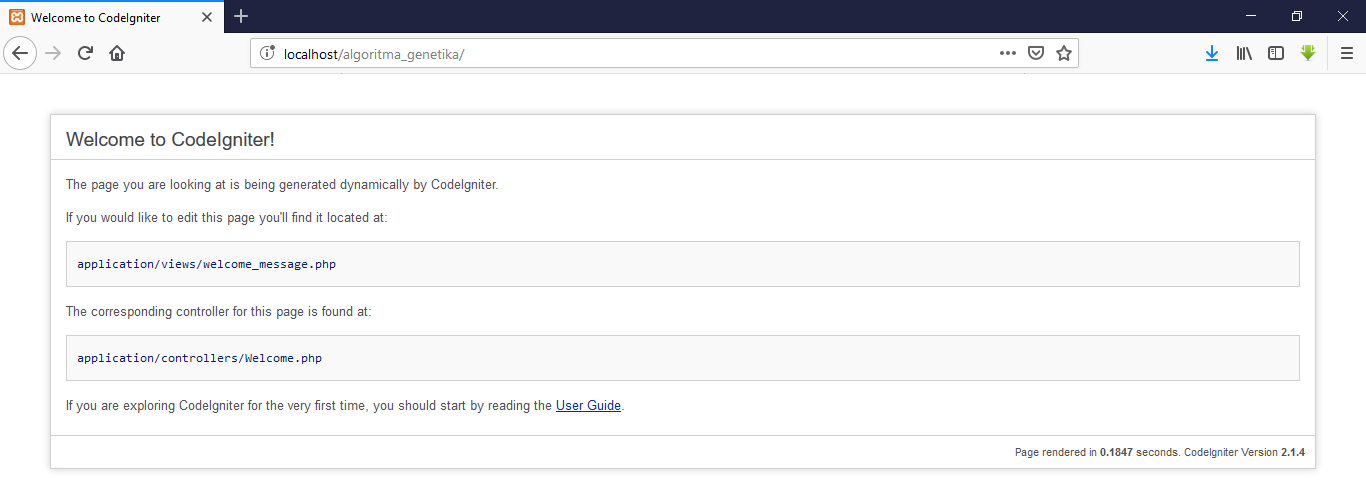
\includegraphics[width=0.5\textwidth]{figures/CodeIgniter1.PNG}
    		\label{CodeIgniter1}
		\end{figure}
    \end{enumerate}
    
\section{Struktur CodeIginter}
\begin{enumerate}
    \item Folder \textbf{Application}, merupakan folder yang pada dasarnya menyimpan aplikasi yang sedang kita buat
    \item Folder \textbf{Cache}, merupakan folder yang menyimpan semua cache yang dibuat oleh cache library
    \item Folder \textbf{Config}, merupakan folder yang menyimpan informasi mengenai konfigurasi aplikasi seperti autoload, database, routes dan lainnya.
    \item Folder \textbf{Controller}, merupakan folder menyimpan controller - controller aplikasi yang dapat digunakan untuk menyusun aktivitas program .
    \item Folder \textbf{Core}, adalah folder untuk memperluas class class inti codeigniter.
    \item Folder \textbf{Helpers}, merupakan folder untuk menyimpan helpers.
    \item Folder \textbf{Hooks}, merupakan folder untuk menyimpan hooks untuk mengubah alur fungsi dari core Codeigniter
    \item Folder \textbf{Language}, merupakan folder untuk menyimpan bahasa - bahasa yang akan digunakan.
    \item Folder \textbf{Libraries}, merupakan folder untuk menyimpan library.
    \item Folder \textbf{Logs}, merupakan folder untuk menyimpan semua error log apabila error log diaktifkan.
    \item Folder \textbf{Models}, merupakan folder untuk menyimpan models yang akan mendefinisikan tabel dari database yang dapat kita gunakan oleh Controller yang kita buat untuk mengakses database.
    \item Folder \verb|third_party|, merupakan folder untuk menyimpan fungsi fungsi tambahan dalam cara kerja codeigniter.
    \item Folder \textbf{Views}, merupakan folder untuk menyimpan tampilan dari aplikasi yang kita buat.
    \item Folder \textbf{System}, merupakan folder untuk menyimpan sistem inti dari Codeigniter.
\end{enumerate}

\section{Konfigurasi CodeIgniter 3}
Di dalam folder application/config/ terdapat berbagai macam file konfigurasi yang dapat kita atur sendiri nantinya.
\begin{enumerate}
    \item \textbf{autoload.php}, digunakan untuk menambahkan package, libraries, drivers, helper, atau custom config lainnya agar secara otomatis diload oleh codeigniter.
    \item \textbf{config.php}, digunakan untuk membuat pengaturan dasar untuk web app codeigniter anda, seperti \verb|base_url|, index page, cookie, proxy dan lain lain.
    \item \textbf{constants.php}, digunakan untuk kita dapat membuat constant baru.
    \item \textbf{database.php}, digunakan untuk mengatur koneksi web app kita ke database.
    \item \textbf{doctypes.php}, sebagai tempat penyimpanan deklarasi dokumen Doctype.
    \item \verb|foreign_chars.php|, sebagai tempat penyimpanan karakter karakter asing.
    \item \textbf{hooks.php}, digunakan untuk mendefine "hooks" untuk meng extends CI
    \item \textbf{memcached.php}, config yang memungkinkan kita mencache database, driver dan lain lain sehingga lebih efektif.
    \item \textbf{migration.php}, config yang memungkinkan kita melakukan database migration. Secara default dijadikan False.
    \item \textbf{mimes.php}, menyimpan array yang berisi tipe file untuk fungsi upload.
    \item \textbf{profiler.php}, digunakan untuk mengatur profiler yang berguna pada saat debugging.
    \item \textbf{routes.php}, digunakan untuk mengatur default controllerdan overide 404
    \item \textbf{smileys.php}, menyimpan array yang berisi smiley yang membantu helper emoticon.
    \item \verb|user_agents.php|, menyimpan data user agent, yang membantu class User Agen untuk mengidentifikasi browser, platform, robotdan datamobile device
\end{enumerate}

Pada konfigurasi yang saya lakukan hanya melukakan konfigurasi pada file autoload.php, config.php, database.php dan routes.php. Berikut cara konfigurasinya:
\begin{enumerate}
    \item Autoload.php
		\begin{figure}[!htbp]
    		\centering
    		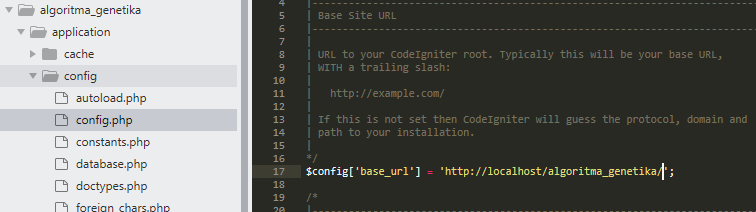
\includegraphics[width=0.5\textwidth]{figures/CodeIgniter2.PNG}
    		\label{CodeIgniter2}
		\end{figure}
		\par Pada file ini saya meng-input libraries untuk support framework CodeIgniter ini terhadap database, \verb|form_validation| yang akan dibuat nantinya, pagination dan Session untuk mengaktifkan session pada CodeIgniter.
        Pada variable autoload helper saya meng-input url dan form semua di inputkan sesuai dengan kebutuhan pembuat aplikasi. Array tersebut akan di eksekusi secara automatis oleh CodeIgniter.

    \item Config.php
		\begin{figure}[!htbp]
    		\centering
    		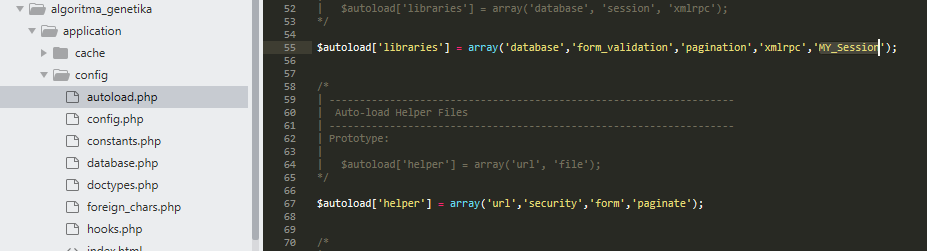
\includegraphics[width=0.5\textwidth]{figures/CodeIgniter3.PNG}
    		\label{CodeIgniter3}
		\end{figure}
        \par Pada config.php inputkan url utama aplikasi pada variable config \verb|base_url| seperti pada gambar diatas.
        
    \item Database.php
		\begin{figure}[!htbp]
    		\centering
    		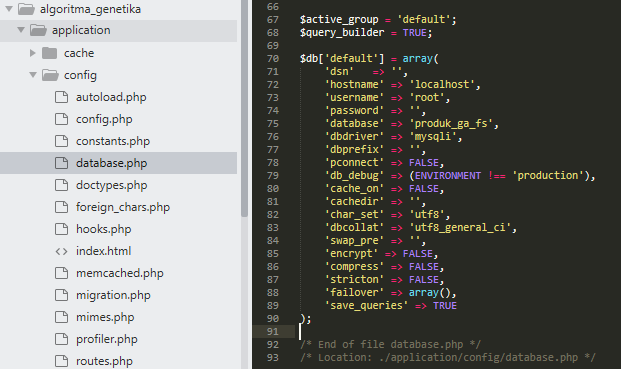
\includegraphics[width=0.6\textwidth]{figures/CodeIgniter4.PNG}
    		\label{CodeIgniter4}
		\end{figure}
		\par Pada database.php konfigurasi yang dilakukan untuk mengkoneksikan database yaitu MySQL dengan aplikasi web berbasis framework CodeIgniter. Dapat dilihat pada line 72, hostname yang diiniputkan sesuai dengan hostname yang dipakai, disini saya menginputkna localhost dengan username default yaitu root password dikosongkan karena pada Xampp saya tidak menggunakan password. Pada database line 75 inputkan nama database sesuai dengan nama database yang ada pada MySQL.
		
	\item Routes.php
		\begin{figure}[!htbp]
    		\centering
    		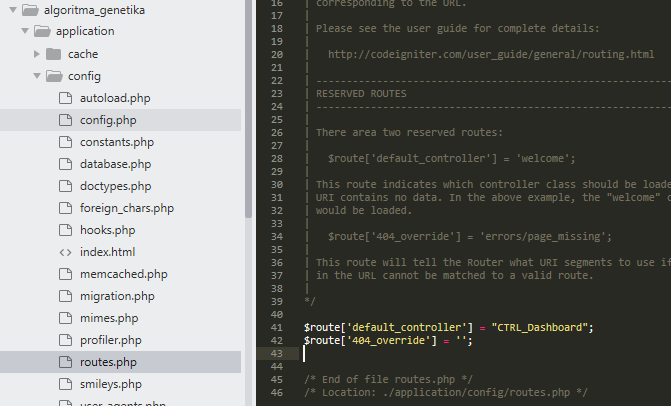
\includegraphics[width=0.7\textwidth]{figures/CodeIgniter5.PNG}
    		\label{CodeIgniter5}
		\end{figure}
		\par Pada file ini dilakukan konfigurasi dimana controller mana yang akan pertama di eksekusi ketika url dijalankan.
\end{enumerate}

\section{Konfigurasi Bootstrap dan Template CodeIgniter 3}
Ada berbagai macam konfigurasi bootstrap dan template terhadap CodeIgniter, baik secara install maupun dengan cara konfigurasi sendiri. Pada tutorial kali ini saya ingin menerapkan bootstrap dan template di CodeIgniter dengan cara cepat. Untuk yang ingin menggunakan cara instan, bisa dengan cara mengunjungi website w3layout.com dan website yang menyediakan assets template dan bootstrap siap pakai. Berikut cara konfigurasi template dan bootstrap pada CodeIgniter:
\begin{enumerate}
    \item Siapkan template bootstrap yang sudah didownload
    \item Extrak file tersebut jika dalam bentuk .rar atau .zip
    \item Buat folder baru dengan nama assets terhadap aplikasi yang ingin di konfigurasi kemudian copy file hasil extrak tadi ke dalam folder tersebut.
		\begin{figure}[!htbp]
    		\centering
    		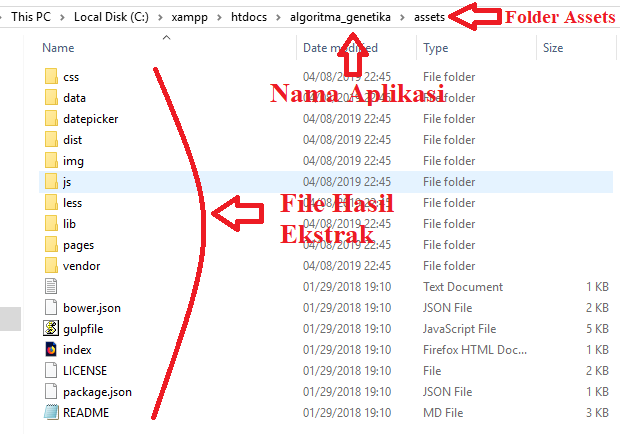
\includegraphics[width=0.5\textwidth]{figures/TBCI1.png}
    		\label{TBCI1}
		\end{figure}
		
	\item Setelah menkopi file kedalam folder assets, langkas selanjutnya adalah memanggil config tersebut. Jangan lupa untuk membuat header dan footer ketika membuat website guna untuk mempermudah apabila terjadi perubahan terhadap beberapa menu.
	\item Copy isi dari index.html yang ada dalam assets kemudian buat file di dalam application/views/namafile.php dengan format .php dan pastekan dalam file tersebut.
	\item Kemudian pisahkan antara header dan footer aplikasi anda.
	\item Pertama lakukan konfigurasi terhadap header dengan cara memanggil link dan script yang sudah di copy di dalam assets, berikut contoh pemanggilanya:
		\begin{figure}[!htbp]
    		\centering
    		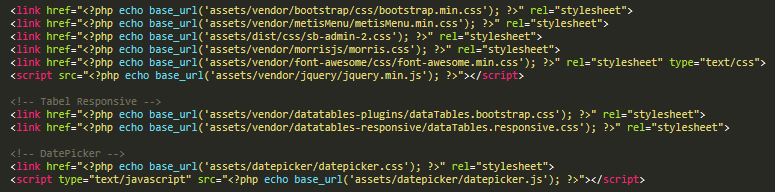
\includegraphics[width=0.5\textwidth]{figures/TBCI2.PNG}
    		\label{TBCI2}
		\end{figure}
		\par Lakukan pemanggilan terhadap semua code yang berbau href dan src dengan mengisikan kodingan seperti echo \verb|base_url|/assets/linkygdituju, terlihat seperti gambar diatas. Lakukan hal yang sama terhadap footer.php. Setelah itu simpan.
		
	\item Selanjutnya membuat file untuk tampilan awal yaitu index.php atau dashboard.php
	\item Edit beberapa codingan yang sudah dipastekan tadi dari assets/index.html ke application/views/index.php sesuai dengan tampilan yang diinginkan. Apabila memisahkan header dan footer jangan lupa untuk memanggil header footer tersebut dengan cara berikut:
		\begin{figure}[!htbp]
    		\centering
    		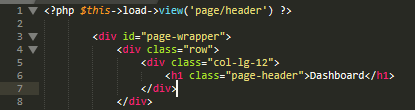
\includegraphics[width=0.5\textwidth]{figures/TBCI4.PNG}
    		\label{TBCI4}
		\end{figure}
	    \par Load view berarti meload file yang ada di dalam folder view dalam artian codingan diatas akan meload file header yang ada di folder application/views/page/header. Simpan semua konfigurasi dan coba jalankan.
	    
    \item Berikut tampilan yang saya modifikasi dari index.html menjadi dashboard.php
		\begin{figure}[!htbp]
    		\centering
    		\caption{Tampilan Awal Template / Bootsrap CodeIgniter 3}
    		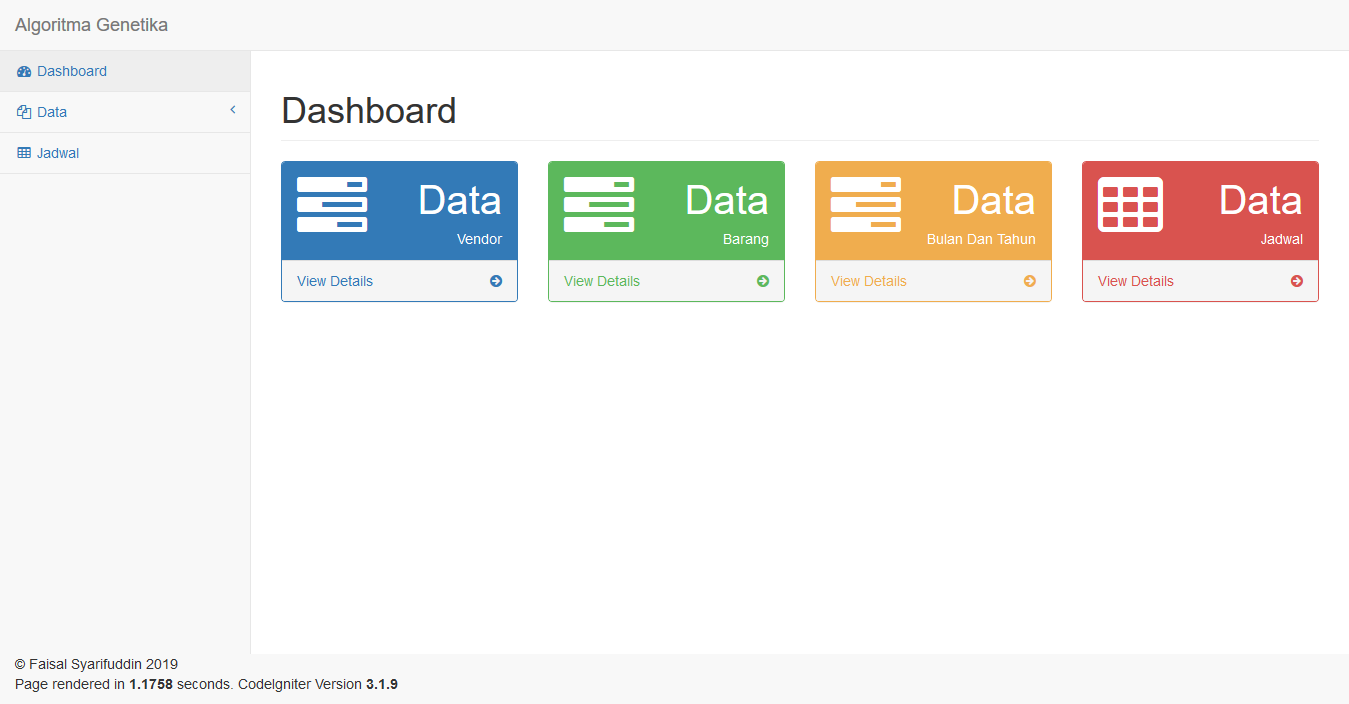
\includegraphics[width=0.5\textwidth]{figures/TBCI3.png}
    		\label{TBCI3}
		\end{figure}
\end{enumerate}

\section{MVC dan CRUD CodeIgniter 3}
\begin{enumerate}
    \item Konfigurasi Model
    \begin{enumerate}
        \item Buat table sesuai dengan kebutuhan aplikasi
        \item Kemudian buat file baru dengan format .php pada application/models
        \item Pastekan codingan dibawah ini
            \par \verb|<?php|\par
            \verb|class MDL_Barang extends CI_Model{|\par
            \verb|function __construct(){|\par
            \verb|parent::__construct();|\par
            \verb|}|\par
            \verb|public function get_barang(){|\par
            \verb|$hasil=$this->db->get('barang');|\par
            \verb|if($hasil->num_rows() > 0){|\par
            \verb|return $hasil->result();|\par
            \verb|}else{|\par
            \verb|return false;|\par
            \verb|}|\par
            \verb|}|\par
            
            \verb|public function insert_barang($barang_data)|\par
            \verb|{|\par
            \verb|$this->db->insert('barang',$barang_data);|\par
            \verb|}|\par
            
            \verb|public function find_barang($kode_barang)|\par
            \verb|{|\par
            \verb|$hasil = $this->db->where('kode_barang',$kode_barang)->limit(1)->get('barang');|\par
            \verb|if($hasil->num_rows() > 0){|\par
            \verb|return $hasil->row();|\par
            \verb|}else{|\par
            \verb|return array();|\par
            \verb|}|\par
            \verb|}|\par
            
            \verb|public function update_barang($kode_barang, $barang_data)|\par
            \verb|{|\par
            \verb|$this->db->where('kode_barang',$kode_barang)|\par
            \verb|->update('barang',$barang_data);|\par
            \verb|}|\par
            	
            \verb|public function delete_barang($kode_barang)|\par
            \verb|{|\par
            \verb|$this->db->where('kode_barang',$kode_barang)|\par
            \verb|->delete('barang');|\par
            \verb|}|\par
            
            \verb|public function detail_barang($kode_barang)|\par
            \verb|{|\par
            \verb|$hasil = $this->db->where('kode_barang',$kode_barang)->limit(1)->get('barang');|\par
            \verb|if($hasil->num_rows() > 0){|\par
            \verb|return $hasil->result();|\par
            \verb|}else{|\par
            \verb|return array();|\par
            \verb|}|\par
            \verb|}|\par
            \verb|}|\par

        \par Penjelasan:
        \begin{enumerate}
            \item function \verb|get_barang| berfungsi untuk meload semua data yang ada di database barang
            \item function \verb|insert_barang| berfungsi untuk melakukan execute insert data ke dalam table barang
            \item function \verb|find_barang| berfungsi untuk mencari kode barang yang akan di edit
            \item function \verb|update_barang| berfungsi untuk melakukan execute update terhadap table barang
            \item function \verb|delete_barang| berfungsi untuk melakukan execute delete data pada table barang
            \item function \verb|detail_barang| berfungsi untuk melihat data lengkap barang sesuai dengan id yang dipanggil.
            
            \par Function-function di atas merupakan function dasar untuk melakukan proses CRUD di model CodeIgniter 3.
        \end{enumerate}
    \end{enumerate}
    \item Konfigurasi Controller
    \begin{enumerate}
        \item Buat file baru dengan format .php di folder application/controller, kemudian buat beberapa function crud
        \item Function pertama adalah function \verb|index_barang|, untuk menampilakn seluruh data yang ada pada table barang
    		\begin{figure}[!htbp]
        		\centering
        		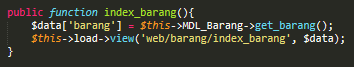
\includegraphics[width=0.5\textwidth]{figures/Controller1.PNG}
        		\label{Controller1}
    		\end{figure}
    		
        \item Function kedua yaitu function \verb|add_barang|, untuk melakukan proses input data dalam bentuk variable sesuai dengan field yang ada pada table barang  yang kemudian variable tersebut akan di lempar ke model untuk di inputkna kedalam table
    		\begin{figure}[!htbp]
        		\centering
        		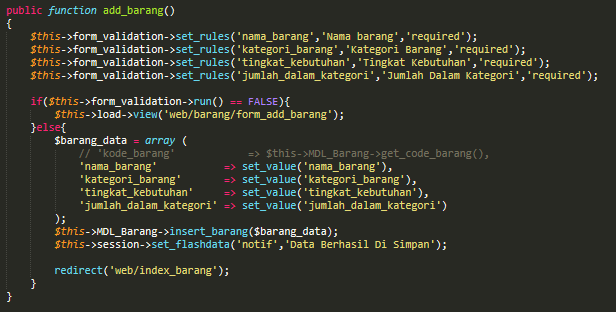
\includegraphics[width=0.5\textwidth]{figures/Controller2.PNG}
        		\label{Controller2}
    		\end{figure}
    		
    	\item Selanjutnya function \verb|edit_barang|, untuk melakukan proses edit data barang yang kemudian variable yang di tampung akan di execute pada model function \verb|update_barang|
    		\begin{figure}[!htbp]
        		\centering
        		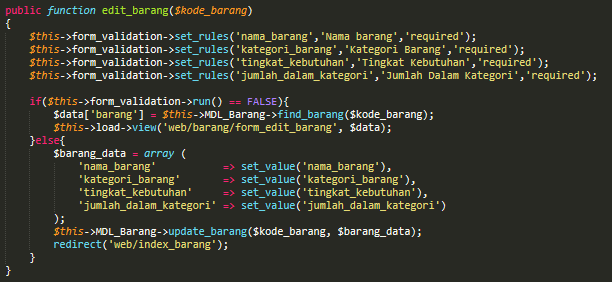
\includegraphics[width=0.5\textwidth]{figures/Controller3.PNG}
        		\label{Controller3}
    		\end{figure}
    		
    	\item Function \verb|delete_barang|, untuk melakukan hapus data berdasarkan id yang di execute
    		\begin{figure}[!htbp]
        		\centering
        		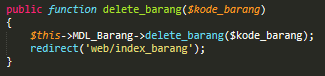
\includegraphics[width=0.5\textwidth]{figures/Controller4.PNG}
        		\label{Controller4}
    		\end{figure}
    \end{enumerate}
    
    \item Konfigurasi Views
    \begin{enumerate}
        \item Buat file  baru pada application/views dengan format .php kemdian buat desain untuk meanmpilakn data dari table barang, berikut contoh codingan untuk vies data barang
    		\begin{figure}[!htbp]
        		\centering
        		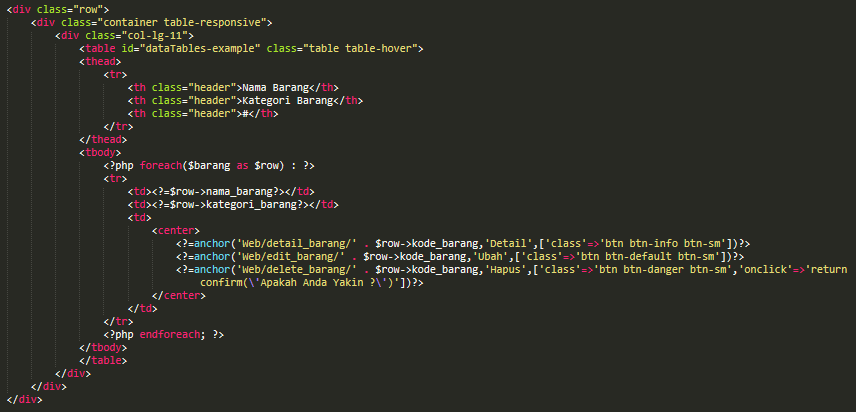
\includegraphics[width=0.7\textwidth]{figures/Views1.PNG}
        		\label{Views1}
    		\end{figure}
    		
    	\item Buat file baru lagi untuk view tambah barang
    		\begin{figure}[!htbp]
        		\centering
        		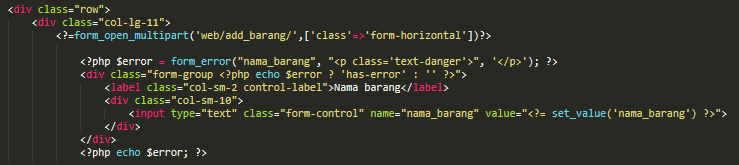
\includegraphics[width=0.6\textwidth]{figures/Views2.PNG}
        		\label{Views2}
    		\end{figure}
    		\par Jangan lupa untuk menutup form dan pastikan name pada codingan views sesuai dengan data variable yang akan di execute pada function \verb|add_barang|
    		
    	\item Kemudian buat file baru untuk views edit data barang, pada edit barang, hal pertama yang harus dilakukan setelah menekan tombol edit barang adalah memanggil semua data yang ada pada table agar dapat diedit, berikut contoh pemanggilan data pada form edit data barang
    		\begin{figure}[!htbp]
        		\centering
        		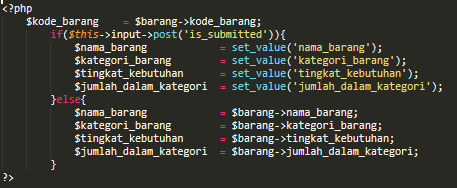
\includegraphics[width=0.5\textwidth]{figures/Views3.PNG}
        		\label{Views3}
    		\end{figure}
    		\par Setelah memanggil dibawah codingan tersebut buat form untuk view edit data barang
    		\begin{figure}[!htbp]
        		\centering
        		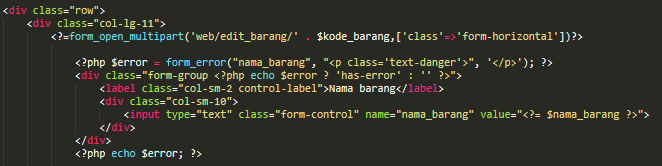
\includegraphics[width=0.5\textwidth]{figures/Views4.PNG}
        		\label{Views4}
    		\end{figure}
    		\par Pastikan value terisi agar saat melakukan edit data yang diedit dapat terlihat dan pastikan pada name sesuai dengan field yang ada pada table dan function \verb|edit_barang|
    		
    	\item Simpan semua file tersebut dan jalankan aplikasi. Berikut tampilan CRUD dari codingan yang di buat
    		\begin{figure}[!htbp]
        		\centering
        		\caption{Tampilan Hasil MVC dan CRUD}
        		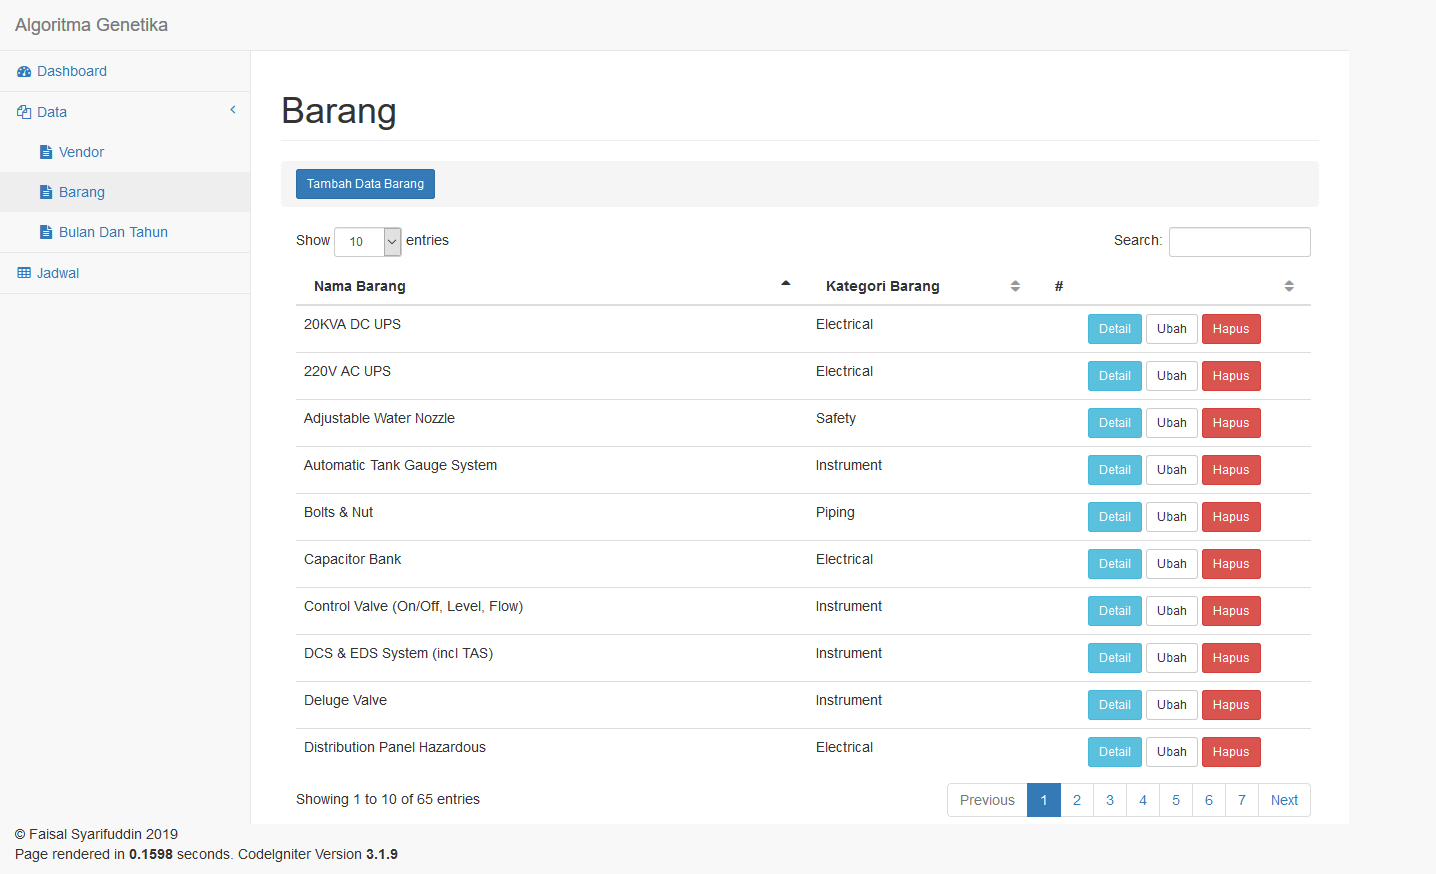
\includegraphics[width=0.5\textwidth]{figures/Views5.png}
        		\label{Views5}
    		\end{figure}
    \end{enumerate}
\end{enumerate}